\documentclass[9pt,twocolumn,twoside,]{pnas-new}

% Use the lineno option to display guide line numbers if required.
% Note that the use of elements such as single-column equations
% may affect the guide line number alignment.


\usepackage[T1]{fontenc}
\usepackage[utf8]{inputenc}

% tightlist command for lists without linebreak
\providecommand{\tightlist}{%
  \setlength{\itemsep}{0pt}\setlength{\parskip}{0pt}}


% Pandoc citation processing
\newlength{\cslhangindent}
\setlength{\cslhangindent}{1.5em}
\newlength{\csllabelwidth}
\setlength{\csllabelwidth}{3em}
\newlength{\cslentryspacingunit} % times entry-spacing
\setlength{\cslentryspacingunit}{\parskip}
% for Pandoc 2.8 to 2.10.1
\newenvironment{cslreferences}%
  {}%
  {\par}
% For Pandoc 2.11+
\newenvironment{CSLReferences}[2] % #1 hanging-ident, #2 entry spacing
 {% don't indent paragraphs
  \setlength{\parindent}{0pt}
  % turn on hanging indent if param 1 is 1
  \ifodd #1
  \let\oldpar\par
  \def\par{\hangindent=\cslhangindent\oldpar}
  \fi
  % set entry spacing
  \setlength{\parskip}{#2\cslentryspacingunit}
 }%
 {}
\usepackage{calc}
\newcommand{\CSLBlock}[1]{#1\hfill\break}
\newcommand{\CSLLeftMargin}[1]{\parbox[t]{\csllabelwidth}{#1}}
\newcommand{\CSLRightInline}[1]{\parbox[t]{\linewidth - \csllabelwidth}{#1}\break}
\newcommand{\CSLIndent}[1]{\hspace{\cslhangindent}#1}


\templatetype{pnasresearcharticle}  % Choose template

\title{Template for preparing your research report submission to PNAS
using RMarkdown}

\author[a,1]{Gabrielle Bibeau}
\author[a]{Laura Glaude}
\author[a]{Emmanuelle Langlois}
\author[a]{Cloé Tanguay}

  \affil[a]{Université de Sherbrooke, Département de Biologie, 2500
Boulevard de l'Université, Sherbrooke, Québec, Canada}


% Please give the surname of the lead author for the running footer
\leadauthor{Anonymous}

% Please add here a significance statement to explain the relevance of your work
\significancestatement{Authors must submit a 120-word maximum statement
about the significance of their research paper written at a level
understandable to an undergraduate educated scientist outside their
field of speciality. The primary goal of the Significance Statement is
to explain the relevance of the work in broad context to a broad
readership. The Significance Statement appears in the paper itself and
is required for all research papers.}


\authorcontributions{Please provide details of author contributions
here.}



\correspondingauthor{\textsuperscript{1} À qui la correspondance devrait
être addressée. Courriel:
\href{mailto:bibg1101@usherbrooke.ca}{\nolinkurl{bibg1101@usherbrooke.ca}}}

% Keywords are not mandatory, but authors are strongly encouraged to provide them. If provided, please include two to five keywords, separated by the pipe symbol, e.g:
 \keywords{  Benthos |  Biodiversité  } 

\begin{abstract}
Please provide an abstract of no more than 250 words in a single
paragraph. Abstracts should explain to the general reader the major
contributions of the article. References in the abstract must be cited
in full within the abstract itself and cited in the text.
\end{abstract}

\dates{This manuscript was compiled on \today}
\doi{\url{www.pnas.org/cgi/doi/10.1073/pnas.XXXXXXXXXX}}

\begin{document}

% Optional adjustment to line up main text (after abstract) of first page with line numbers, when using both lineno and twocolumn options.
% You should only change this length when you've finalised the article contents.
\verticaladjustment{-2pt}



\maketitle
\thispagestyle{firststyle}
\ifthenelse{\boolean{shortarticle}}{\ifthenelse{\boolean{singlecolumn}}{\abscontentformatted}{\abscontent}}{}

% If your first paragraph (i.e. with the \dropcap) contains a list environment (quote, quotation, theorem, definition, enumerate, itemize...), the line after the list may have some extra indentation. If this is the case, add \parshape=0 to the end of the list environment.

\acknow{Merci à Victor Cameron et Benjamin Mercier sans qui ce projet
n'aurait été possible.}

========================================

Dans le contexte actuel de constantes variations climatiques,
conséquences des changements climatiques, il est primordial d'analyser
les réactions de la biodiversité face à de telles variations afin d'être
en mesure de mieux la comprendre et ainsi, de mieux la protéger. C'est
pourquoi, dans le cadre d'un suivi annuel de la biodiversité benthique
de ruisseaux, cette étude se penchera sur l'influence des variations
spatiales et temporelles sur la structure des communautés de milieux
lotiques. L'objectif est d'évaluer l'impact de différentes variables
abiotiques environnementales sur la richesse spécifique benthique de
ruisseaux. Pour ce faire, cinq variables environnementales seront prises
en compte sur différents sites : la profondeur et la largeur du cours
d'eau, la transparence de son eau, sa température ainsi que la vitesse
du courant.

\hypertarget{muxe9thodes}{%
\subsubsection*{Méthodes}\label{muxe9thodes}}
\addcontentsline{toc}{subsubsection}{Méthodes}

Le jeu de données utilisé contient une partie des inventaires du benthos
faits par le ministère de l'Environnement, de la Lutte contre les
Changements Climatiques, de la Faune et des Parcs (MELCCFP) avec le
protocole d'échantillonnage des macroinvertébrés benthiques d'eau douce
du Québec dans le cadre du suivi de la qualité de l'eau des rivières du
Québec. Ces données, extraites du site Biodiversité Québec, recensent
les espèces de macroinvertébrés benthiques dans les rivières du Québec.

Avant l'analyse des données, celles-ci sont passées à travers plusieurs
manipulations. Premièrement, les données, extraites sous forme de
fichiers .csv, ont été manipulées pour être regroupées en une matrice.
Deuxièmement, la matrice a été nettoyée, notamment en assignant une
classe pertinente aux valeurs de la matrice (ex: les dates en format
`Date' et non en format `Character'), en enlevant les colonnes
importunes (ne contenant que des NAs ou étant des doublons) et en
remplaçant les données problématiques par des NAs (valeurs de -99 pour
des variables strictement positives dans la réalité). Troisièmement, des
numéros d'identification (IDs) ont été assignés pour toutes les
combinaisons de dates, de sites et d'heures. Finalement, une base de
données .db a été créée pour entreposer deux tables : une contenant des
informations reliées aux IDs et l'autre, des informations sur les
abondances des taxons de benthos.

Différentes analyses ont été performées sur les données pour répondre
aux questions posées par ce rapport. D'abord, des régressions linéaires
simples (p=0.05) de la richesse spécifique ont été produites en fonction
des variables suivantes : la largeur de la rivière, la profondeur de la
rivière, la vitesse du courant et la température de l'eau. Ensuite, un
diagramme à moustache validé par un test de t avec un intervalle de
confiance de 0.95 a été réalisé pour la richesse spécifique en fonction
de la transparence de l'eau. Puis, une vérification d'interactions pour
toutes les combinaisons possibles de variables abiotiques a été conduite
avec des régressions linéaires simples (p=0.05). Seule la température de
l'eau a une distribution normale. Suite à des tests de régressions
linéaires généralisées avec différentes familles (par exemple Poisson),
nous avons conclu que les erreurs avaient une distribution plus normale
lorsque nous utilisions la régression linéaire simple. Finalement, une
ordination de type PCoA (Principal Coordinates Analysis) de la
composition en abondance des communautés benthiques a été produite
seulement avec les échantillons pris plus d'une fois sur un même site.
Aucun test statistique n'a été réalisé pour valider les observations
permises par cet outil de visualisation.

\hypertarget{ruxe9sultats}{%
\subsubsection*{Résultats}\label{ruxe9sultats}}
\addcontentsline{toc}{subsubsection}{Résultats}

Nous avons d'abord testé l'effet des différentes variables abiotiques
(largeur de la rivière, profondeur de la rivière, transparence de l'eau,
température de l'eau et vitesse du courant) sur la richesse spécifique
des échantillons analysés. Les régressions linéaires à la figure
\ref{fig:regression_richesse} nous permettent d'observer un effet
significatif pour la variable de la température, mais pas pour les
autres.

\begin{figure}
\centering
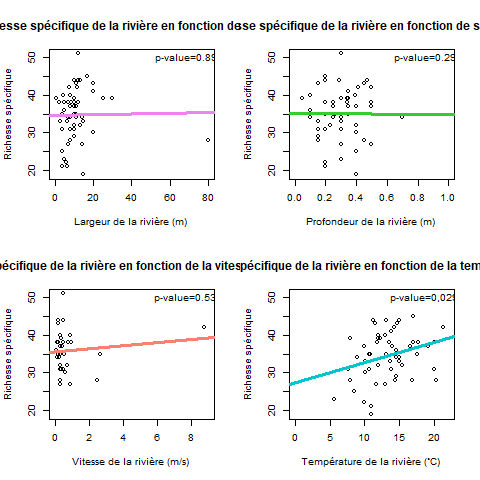
\includegraphics{regression_richesse.png}
\caption{Régressions linéaires de la richesse en fonction de (A) la
largeur de la rivière, (B) la profoncdeur de la rivière, (C) la vitesse
du courant et (D) la température de l'eau.
\label{fig:regression_richesse}}
\end{figure}

L'effet de la transparence a été visualisé en diagramme à moustache
(Figure \ref{fig:boxplot_richesse}). Il s'avère que cette variable
n'affecte pas non plus significativement la richesse spécifique des
communautés de benthos.

\begin{figure}
\centering
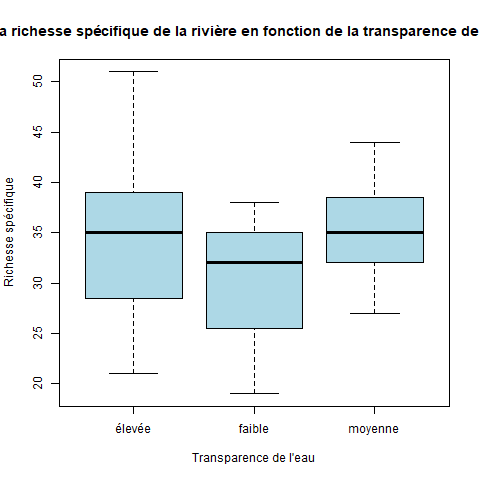
\includegraphics{boxplot_richesse.png}
\caption{Diagramme à moustache de la richesse spécifique des
échantillons de benthos en fonction de la transparence de l'eau lors de
l'échantillonnage. \label{fig:boxplot_richesse}}
\end{figure}

Ensuite, nous avons vérifié s'il y avait des interactions entre les
variables. Selon le tableau de la figure \ref{fig:tableau_interaction},
il n'y a aucune interaction significative entre les variables abiotiques
en ce qui concerne la richesse spécifique des échantillons.

\begin{figure}
\centering
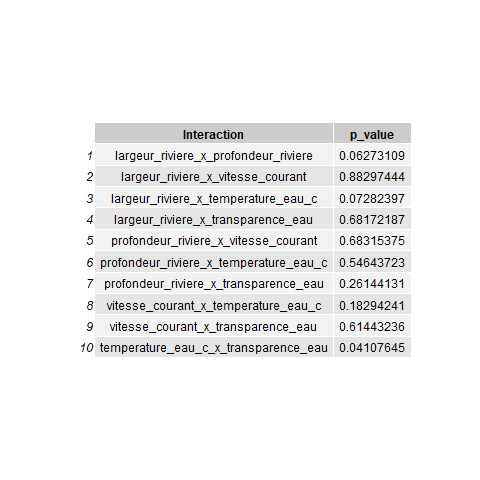
\includegraphics{tableau_interaction.png}
\caption{Tableau de la significativité des interactions entre les
variables affectant la richesse spécifique des échantillons dans des
régressions linéaires. \label{fig:tableau_interaction}}
\end{figure}

Finalement, la diversité beta a été observée à l'aide d'une ordination
PCoA. À l'oeil, sur la figure \ref{fig:ordination_sites}, certains sites
semblent avoir des commuanutés de benthos similaires entre les
différentes périodes d'échantillonnages, alors que d'autres sont plutôt
variées. Entre eux, les sites sont parfois très proches en termes de
composition même s'ils sont différents géographiquement, d'autres fois
complètement différents.

\begin{figure}
\centering
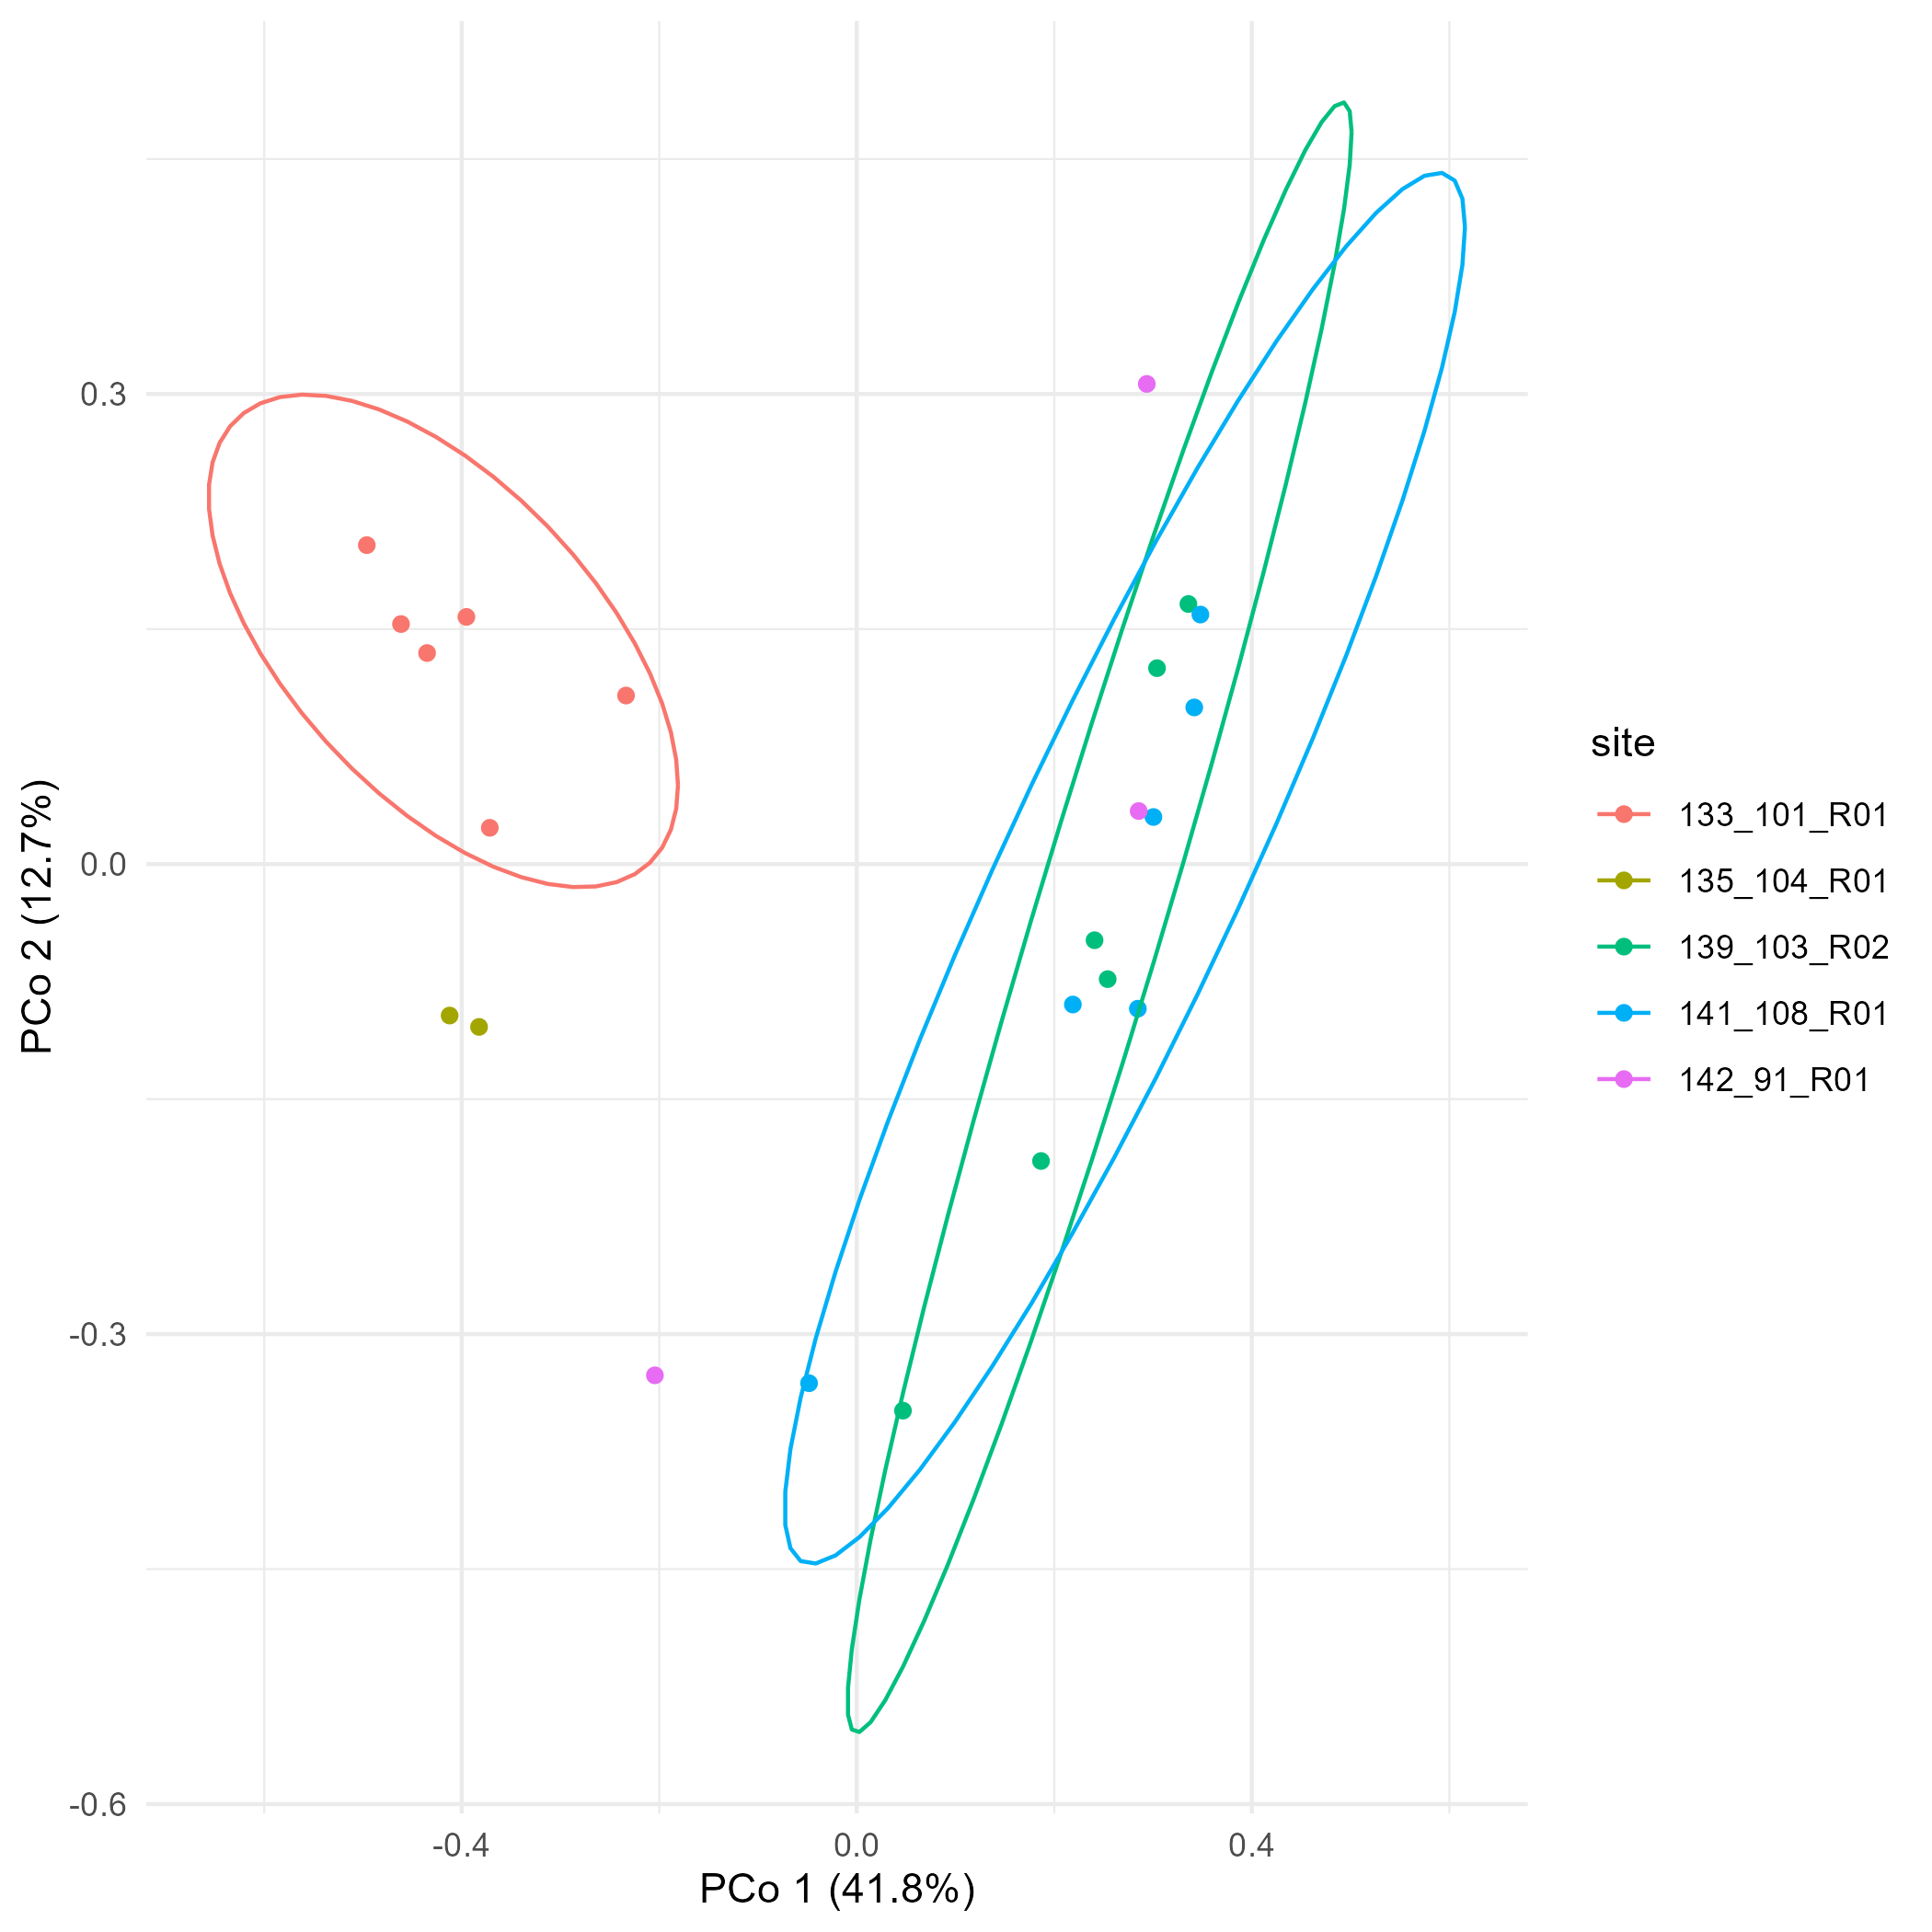
\includegraphics{ordination_sites.png}
\caption{PCoA des communautés de benthos échantillonnées par
Biodiversité Québec en fonction du site. \label{fig:ordination_sites}}
\end{figure}

\hypertarget{discussion}{%
\subsubsection*{Discussion}\label{discussion}}
\addcontentsline{toc}{subsubsection}{Discussion}

Les résultats de l'étude offrent une vision limitée des variables qui
influent sur la diversité du benthos. Mise à part la température, aucun
facteur d'habitat n'a révélé de résultats significatifs. La littérature
souligne l'impact clair de la température sur les communautés
benthiques, mais l'effet des autres variables reste incertain (Jowett
2003; Godson, Vincent, and Krishnakumar 2022).Bien qu'une relation entre
la vélocité, la largeur et la profondeur des rivières ait été démontrée
dans d'autres études, elle ne semble pas s'appliquer aux petits cours
d'eau (Jowett 2003; Godson, Vincent, and Krishnakumar 2022). De plus, la
vélocité devrait être mesurée au niveau du substrat, l'espace occupé par
le benthos, plutôt que dans la colonne d'eau, ce qui pourrait expliquer
le manque de résultats significatifs (Jowett 2003; Godson, Vincent, and
Krishnakumar 2022). En outre, plusieurs variables importantes, telles
que les caractéristiques du substrat, n'ont pas été testées en raison de
l'absence de données (Jowett 2003; Godson, Vincent, and Krishnakumar
2022). D'autres caractéristiques de l'habitat peuvent également
influencer la structure des populations d'invertébrés benthiques
lorsqu'elles sont mises en relation avec les caractéristiques des
sédiments (Jowett 2003; Godson, Vincent, and Krishnakumar 2022). Il
serait donc pertinent d'ajouter ces mesures au protocole de
caractérisation du milieu dans les futures études. De plus, les tests
ont été effectués sur un échantillon limité de données de benthos, ce
qui peut avoir réduit notre capacité à obtenir des résultats
significatifs. Augmenter la quantité de données pourrait donc accroître
nos chances de détection de relations significatives.

En ce qui concerne les interactions entre les variables abiotiques, nos
résultats montrent qu'aucune interaction significative n'a été observée
concernant la richesse spécifique des échantillons. Cela pourrait être
attribué à la sensibilité limitée de la méthode utilisée pour détecter
ces interactions, en raison de considérations telles que les méthodes de
sélection de variables et les approches de sélection de modèles
Claeskens (2016).

Enfin, en ce qui concerne l'ordination, nos résultats révèlent que
certains sites présentent des communautés de benthos similaires à
travers différentes périodes d'échantillonnage, tandis que d'autres
présentent une plus grande variabilité. Malgré des différences
géographiques, certains sites ont une composition similaire, tandis que
d'autres sont distincts les uns des autres. Cette observation pourrait
s'expliquer par le fait que la similarité des communautés écologiques
diminue avec la distance, mais des facteurs tels que l'échelle spatiale,
les propriétés des organismes, la région d'étude et l'écosystème peuvent
influencer cette relation pour rendre des sites semblables entre eux
malgré la distance qui les sépare Soininen, McDonald, and Hillebrand
(2007).

\showmatmethods
\showacknow
\pnasbreak

\hypertarget{refs}{}
\begin{CSLReferences}{1}{0}
\leavevmode\vadjust pre{\hypertarget{ref-claeskens_statistical_2016}{}}%
Claeskens, Gerda. 2016. {``Statistical {Model} {Choice}.''} \emph{Annual
Review of Statistics and Its Application} 3 (March).
\url{https://doi.org/10.1146/annurev-statistics-041715-033413}.

\leavevmode\vadjust pre{\hypertarget{ref-godson_ecology_2022}{}}%
Godson, Prince S., Salom Gnana Thanga Vincent, and S. Krishnakumar.
2022. \emph{Ecology and {Biodiversity} of {Benthos}}. San Diego, UNITED
STATES: Elsevier.
\url{http://ebookcentral.proquest.com/lib/usherbrookemgh-ebooks/detail.action?docID=6940166}.

\leavevmode\vadjust pre{\hypertarget{ref-jowett_hydraulic_2003}{}}%
Jowett, I. G. 2003. {``Hydraulic Constraints on Habitat Suitability for
Benthic Invertebrates in Gravel-Bed Rivers.''} \emph{River Research and
Applications} 19 (5-6): 495--507. \url{https://doi.org/10.1002/rra.734}.

\leavevmode\vadjust pre{\hypertarget{ref-soininen_distance_2007}{}}%
Soininen, Janne, Robert McDonald, and Helmut Hillebrand. 2007. {``The
Distance Decay of Similarity in Ecological Communities.''}
\emph{Ecography} 30 (1): 3--12.
\url{https://doi.org/10.1111/j.0906-7590.2007.04817.x}.

\end{CSLReferences}



% Bibliography
% \bibliography{pnas-sample}

\end{document}
